% !TeX root = main.tex

\chapter{Long Short Term Memory}

Objectif principal de ce projet, l'architecture neuronale Long Short Term Memory
(LSTM) est décrite dans cette partie. Tout comme les autres architectures
neuronales, elle est constituée d'un assemblage de blocs élémentaires qui
disposent d'un ensemble de variables, appelés poids, à adapter lors de la phase
d'apprentissage afin de reproduire une fonction. Cependant, la cellule
élémentaire d'un réseau LSTM est bien plus complexe que celle d'un réseau
neuronal à perceptrons. \\

La dénomination LSTM vient du fait que ce type de réseau possède une mémoire de
plus longue durée que des structures plus simples avec une seule couche de neurones.
Ainsi, il sera possible d'apprendre des fonctions telles que la grammaire de Reber
double, ou bien de générer du texte après avoir appris des écrits de Shakespeare. \\
LSTM est notamment utilisé dans des applications de reconnaissance vocale.

\section{Théorie}
\subsection{Cellule LSTM}
La cellule LSTM est un petit réseau de perceptrons récurrent présentant des
élément nommés en fonction de leur rôle dans la cellule.

\begin{figure}[!ht]
\begin{center}
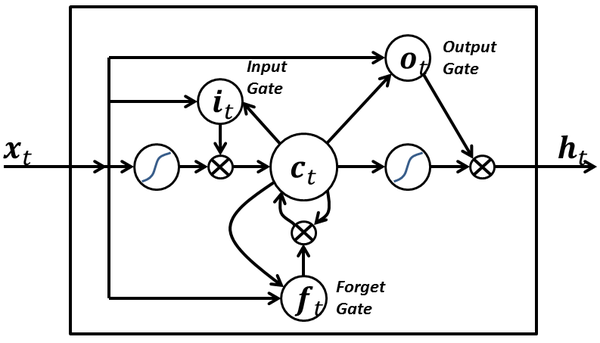
\includegraphics[scale=0.8]{images/lstm.png}
\end{center}
\caption{Cellule LSTM}
\end{figure}

\subsection{Propagation}

\subsection{Algorithmes d'apprentissage}
L'algorithme d'apprentissage est un algorithme BPTT appliqué aux cellules
LSTM considérées.

\begin{figure}[!ht]
\begin{center}
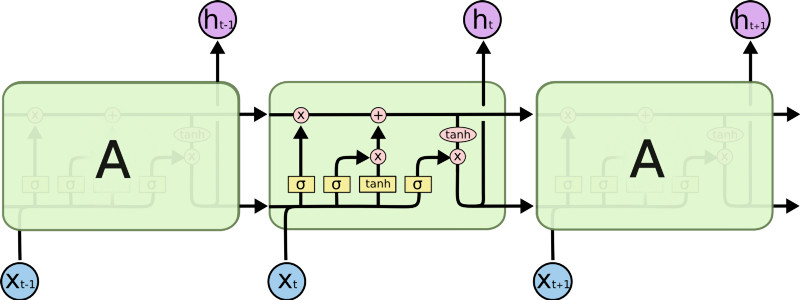
\includegraphics[scale=0.4]{images/lstm-bptt.png}
\end{center}
\caption{Dépliement du temps dans l'espace style BPTT}
\end{figure}

\section{Implémentation}

L'implémenation est effectuée en C++ via la librairie de calcul matriciel
Eigen3. Toutes les matrices sont des objets de type Eigen::MatrixXd (matrice de
double) et les vecteurs des objets de type Eigen::VectorXd.

\medskip

L'aléatoire utilisé est celui natif en C et C++ : rand.
La génération de la graine se fait à partir du temps à la milliseconde pour
éviter une initialisation déterministe dans le cas de l'execution de plusieurs
runs consécutifs. Pour cela la librairie 'sys/time.h' est utilisée, avec un
appel propre aux systèmes UNIX.

\bigskip

\subsection{Structure de données}

Le code se décompose en plusieurs éléments : 

\medskip

\begin{itemize}

  \item Les poids LSTM
  \item La cellule LSTM
  \item Le réseau LSTM

\end{itemize}
\subsubsection{Les poids LSTM}

La classe poids regroupe toutes les matrices de poids des différents noeuds
de la cellule LSTM. Ces dernier sont : input\_gate, input\_block, output\_gate.
Pour chacun des noeuds il existe deux matrices de poids : une relative à
la sortie précédente de la cellule, et l'autre relative à l'entrée de la
cellule. Enfin, il existe aussi pour chaque noeud un vecteur de biais.

\medskip

Tous ces éléments sont amenés à être modifiés, c'est pourquoi l'on crée pour
chacun une matrice (ou un vecteur) de delta : modifications à appliquer.

\medskip

Enfin, les méthodes de l'objet poids LSTM sont le constructeur et
l'application des variations de poids (qui remet par la même occasion à 0
les delta-poids).

\subsubsection{La cellule LSTM}

La cellule LSTM est l'objet élémentaire du réseau. Elle est créée en prenant
pour arguments un pointeur vers un objet de type poids, et les informations de
dimentions d'entrée et sortie.

\medskip

Elle dispose des méthodes nécessaires à la propagation et la rétropropagation
à travers une cellule LSTM.
Pour renvoyer plusieurs vecteurs (la sortie, la mémoire) on utilise ici des
std::vector<Eigen::VectorXd> dont chaque case correspond à un vecteur que l'on
souhaite renvoyer.

\medskip

La propagation n'est rien d'autre qu'une application directe des formules de la
propagation à travers une cellule LSTM. Sont stockées certaines valeurs
intermédiaires pertinentes pour éviter leur calcul à nouveau lors de la
rétropropagation.

\medskip

Lors de la rétropropagation, les variations de poids sont calculées et ajoutées
aux attributs delta\_poids de l'objet weightsLSTM. La fonction de cout choisie
est la fonction de coût quadratique (divisée par deux), sa dérivée étant alors
la différence entre sortie obtenue et sortie attendue.

\bigskip

Les attributs sont donc les suivants :

% TODO

Les méthodes sont donc les suivantes :

% TODO

\subsubsection{Le réseau LSTM}

Le réseau LSTM est principalement constitué d'un std::vector<CellLSTM>.
A chaque temps $t_i$, une nouvelle cellule est crée et stockée à l'index i du
vector.

\medskip

La propagation s'effectue cellule par cellule, chaque cellule prenant en entrée
la sortie de la précédente à $t_{i-1}$ ainsi que l'entrée du réseau au temps
$t_i$.

\medskip

De même, la rétropropagation s'effectue de la dernière cellule du vector à
la première.

\bigskip

Les attributs sont donc les suivants :

% TODO

\bigskip

Les méthodes sont donc les suivantes :

% TODO

\section{Résultats}
\subsection{Apprentissage sur un mot}
\subsection{Grammaire de Reber simple}
\subsection{Grammaire de Reber double}
